% GENERATED FROM typst/manual/sections/02_hydrogen_facing_shell_tests.typ BY scripts/typ2tex.py (v1.0.0) — DO NOT EDIT.
% Edit canonical Typst under typst/ and regenerate with: python3 scripts/typ2tex.py --root . --outdir latex

\section{Hydrogen-facing Shell Tests}\label{manual:hydrogen-shell-tests}

\paragraph{Setup and calculation card.}
The declared signed shell ladder generates exact zero-float D0 rational transition
differences and within-series ratios verified independently by reference-engine vectors
\texttt{RC-031} (\texttt{hydrogen\_shell\_exact\_series.csv}) and \texttt{RC-039}
(\texttt{hydrogen\_shell\_dec\_transitions.csv}) across the Lyman, Balmer, and Paschen
series before any external constant or scale enters. Carried wavelength, frequency, and
energy targets remain quarantined external O0 comparisons at
$B_{\mathrm{ext}}=\mathsf{Q}_{\mathrm{ext}}$ sharing each series baseline; their
display precision is not a measurement uncertainty. Full experimental comparison still
requires a source adapter binding exact NIST-ASD / Hydrogen Handbook rows,
observed-versus-Ritz and air-versus-vacuum conventions, uncertainty semantics, and
shared-denominator covariance under \secref{manual:calculation-spine}.

\subsection{Shared hydrogen-facing shell declaration}\label{manual:hydrogen:scope}

\aodnoteblock{Scope}{This section declares a signed shell comparison ladder, derives its exact rational transition differences and series ratios in D0 arithmetic (\texttt{RC-031}, \texttt{RC-039}), and quarantines downstream NIST wavelength, frequency, and energy comparisons at $B_{\mathrm{ext}}=\mathsf{Q}_{\mathrm{ext}}$.}

\aodnoteblock{Data-support class}{Hydrogen shell tests separate D0 exact rational shell-ratio fixtures (\texttt{RC-031}, \texttt{RC-039}) from O0 quarantined spectral observable-map comparisons. Error quantities are shell-ratio or spectral-map residuals.}

\paragraph{Setup.}
Declare the hydrogen-facing shell scope and integer shell family:

\[
\mathbf{a}_H\vdash(F_H,R_H,\partial R_H,\omega_H),\qquad B_H=(\partial F_H,\omega_H),\qquad S_n,\;n\in\mathbb{Z}_{\ge1}.
\]

For the hydrogen-facing comparison records, declare the normalized signed shell-pressure ladder

\[
\hat{P}^D_{S_n}:=-\frac{1}{n^2}.
\]

\paragraph{Derivation.}
For any downward transition $n\to m$ with $n>m$, the released normalized pressure magnitude is

\[
\Delta\hat{P}^D(n\to m):=\hat{P}^D_{S_n}-\hat{P}^D_{S_m}=\frac{1}{m^2}-\frac{1}{n^2}>0,
\]

with signed state change $\hat{P}^D_{S_m}-\hat{P}^D_{S_n}=-\Delta\hat{P}^D(n\to m)$.

\[
\boxed{\text{Hydrogen shell tests use a declared signed comparison ladder.}}
\]

\aodnoteblock{Remark}{The normalized ladder is a manual comparison choice. The main-note pressure definition remains $p^D=C_3\rho^D_{\omega}$.}

\aodnoteblock{Presentation policy}{All A$\Omega$ shell ratios in the spectral tables are exact rational D0 values (\texttt{RC-031}, \texttt{RC-039}). Decimal target ratios, wavelengths, frequencies, and percent errors are quarantined external presentation coordinates; a $z$-score is recorded only when a row carries an explicit uncertainty.}

\begin{figure}[H]
\centering
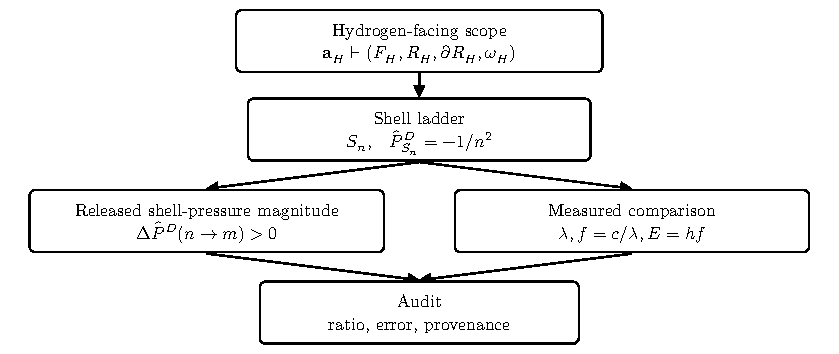
\includegraphics[width=\linewidth]{figures/generated/hydrogen-shell-setup.pdf}
\caption{Hydrogen-facing shell-cycle ladder. The released shell-pressure magnitude is calculated before measured wavelengths and external energy-coordinate comparisons are attached.}
\label{fig:manual-hydrogen-shell-setup}
\end{figure}

\subsection{Shell-radius comparison}\label{manual:hydrogen:radii}

\paragraph{Specialization.}
The shell-radius geometry comparison records the standard quadratic shell scaling

\[
\frac{r_n}{r_1}=n^2.
\]

\begin{table}[H]
\centering
\caption{Hydrogen-facing shell-radius ratios.}
\label{tab:manual-hydrogen-shell-radii}
{\footnotesize
\begin{tabular}{cccc}
\toprule
Shell & A$\Omega$ shell & Ratio target & Status \\
\midrule
$1$ & $S_1$ & $1$ & baseline \\
$2$ & $S_2$ & $4$ & comparison record \\
$3$ & $S_3$ & $9$ & comparison record \\
$4$ & $S_4$ & $16$ & comparison record \\
\bottomrule
\end{tabular}
}
\end{table}

\subsection{Shell-pressure table}\label{manual:hydrogen:pressure-table}

\paragraph{Specialization (\texttt{RC-031}).}
Balmer comparison records fix destination shell $S_2$ ($m=2$). The exact D0 released-pressure
magnitudes and baseline ratios against $3\to2$ (verified in zero-float rational
arithmetic by \texttt{RC-031}, \texttt{hydrogen\_shell\_exact\_series.csv}) are

\[
\Delta\hat{P}^D(n\to2)=\frac{1}{2^2}-\frac{1}{n^2},\qquad\mathcal{R}_{n\to2}=\frac{\Delta\hat{P}^D(n\to2)}{\Delta\hat{P}^D(3\to2)}.
\]

\begin{table}[H]
\centering
\caption{Hydrogen-facing Balmer released-pressure ratios. Targets are ratio comparisons against cited Balmer wavelengths.}
\label{tab:manual-hydrogen-pressure-ratios}
{\footnotesize
\begin{tabular}{cccccc}
\toprule
Line & Transition & $\Delta\hat{P}^D$ & A$\Omega$ ratio & Target ratio & Error [\%] \\
\midrule
H$\alpha$ & $3\to2$ & $5/36$ & $1$ & $1.00000000$ & $0.000000$ \\
H$\beta$ & $4\to2$ & $3/16$ & $27/20$ & $1.34999075$ & $0.000685$ \\
H$\gamma$ & $5\to2$ & $21/100$ & $189/125$ & $1.51198839$ & $0.000768$ \\
H$\delta$ & $6\to2$ & $2/9$ & $8/5$ & $1.59999025$ & $0.000609$ \\
\bottomrule
\end{tabular}
}
\end{table}

\subsection{Shell-energy transitions}\label{manual:hydrogen:energy-transitions}

\paragraph{Quarantined external map.}
Measured frequency and energy coordinates enter strictly downstream under the quarantine
of \appref{manual:external-comparison}. Given a cited vacuum wavelength $\lambda$,

\[
f=\frac{c}{\lambda},\qquad E=h_{\mathrm{ext}}f.
\]

\begin{table}[H]
\centering
\caption{Hydrogen Balmer comparison targets. Wavelength records follow the NIST Atomic Spectra Database target convention.}
\label{tab:manual-hydrogen-balmer-targets}
{\footnotesize
\begin{tabular}{ccccc}
\toprule
Line & Transition & $\lambda_{\mathrm{vac}}$ [nm] & $f$ [Hz] & $E$ [eV] \\
\midrule
H$\alpha$ & $3\to2$ & $656.46$ & $4.56680465\times10^{14}$ & $1.88867865$ \\
H$\beta$ & $4\to2$ & $486.27$ & $6.16514401\times10^{14}$ & $2.54969869$ \\
H$\gamma$ & $5\to2$ & $434.17$ & $6.90495562\times10^{14}$ & $2.85566019$ \\
H$\delta$ & $6\to2$ & $410.29$ & $7.30684292\times10^{14}$ & $3.02186742$ \\
\bottomrule
\end{tabular}
}
\end{table}

\subsection{Hydrogen spectral-series extension}\label{manual:hydrogen:spectral-extension}

\aodnoteblock{Choice}{The Lyman and Paschen records use the same normalized shell-pressure ladder as the Balmer records. The destination shell $S_m$ is declared before each transition table; exact D0 ratio evaluation precedes any quarantined wavelength, frequency, or energy export.}

\paragraph{Derivation.}
For a fixed destination shell $S_m$ and downward transition $n\to m$ ($n>m$),
define the exact D0 A$\Omega$-internal series ratio $R_{\mathrm{series}}(n\to m)=\mathcal{R}_{n\to m,\AO}\ge1$
and its reciprocal baseline-wavelength ratio $\lambda_n/\lambda_{m+1}=1/R_{\mathrm{series}}\le1$:

\[
R_{\mathrm{series}}(n\to m)=\mathcal{R}_{n\to m,\AO}=\frac{\Delta\hat{P}^D(n\to m)}{\Delta\hat{P}^D((m+1)\to m)}\ge1,\qquad\frac{\lambda_n}{\lambda_{m+1}}=\frac{1}{R_{\mathrm{series}}(n\to m)}\le1.
\]

Against quarantined wavelength targets at $B_{\mathrm{ext}}=\mathsf{Q}_{\mathrm{ext}}$,
the inverse-wavelength target ratio is

\[
\mathcal{R}^{\lambda,\mathrm{tar}}_{n\to m}=\frac{\lambda_{(m+1)\to m}}{\lambda_{n\to m}}.
\]

Thus the A$\Omega$-internal pressure ratio $R_{\mathrm{series}}=\mathcal{R}_{n\to m,\AO}\ge1$
compares directly against the measured inverse-wavelength ratio
$\mathcal{R}^{\lambda,\mathrm{tar}}_{n\to m}$, while its reciprocal
$\lambda_n/\lambda_{m+1}=1/R_{\mathrm{series}}\le1$ records the
dimensionless wavelength contraction across the wavelet D.E.C. ledger below.
External frequency-coordinate and energy export remain downstream. The reference engine
(\texttt{manual/data/boundary\_sadar/hydrogen\_shell\_exact\_series.csv}, vector
\texttt{RC-031}) evaluates all Lyman ($m=1$), Balmer ($m=2$), and Paschen ($m=3$)
transitions in reduced exact rational arithmetic prior to quarantined NIST-ASD
wavelength comparison.

\subsubsection{Lyman series}\label{manual:hydrogen:lyman}

For Lyman records, the destination shell is $S_1$. The baseline is $2\to1$, with

\[
\Delta\hat{P}^D(2\to1)=1-\frac{1}{4}=\frac{3}{4}.
\]

\begin{table}[H]
\centering
\caption{Hydrogen Lyman released-pressure ratio audit. Vacuum wavelength targets are downstream comparison records carried by the NIST-ASD target convention.}
\label{tab:manual-hydrogen-lyman-ratios}
{\footnotesize
\begin{tabular}{ccccccc}
\toprule
Line & Transition & $\Delta\hat{P}^D$ & A$\Omega$ ratio & $\lambda_{\mathrm{vac}}$ [nm] & Target ratio & Error [\%] \\
\midrule
Ly$\alpha$ & $2\to1$ & $3/4$ & $1$ & $121.56701$ & $1.00000000$ & $0.000000$ \\
Ly$\beta$ & $3\to1$ & $8/9$ & $32/27$ & $102.57225$ & $1.18518420$ & $0.000083$ \\
Ly$\gamma$ & $4\to1$ & $15/16$ & $5/4$ & $97.2537$ & $1.24999882$ & $0.000095$ \\
Ly$\delta$ & $5\to1$ & $24/25$ & $32/25$ & $94.9740$ & $1.28000305$ & $-0.000239$ \\
Ly$\epsilon$ & $6\to1$ & $35/36$ & $35/27$ & $93.7803$ & $1.29629581$ & $0.000037$ \\
Limit & $\infty\to1$ & $1$ & $4/3$ & series limit & $4/3$ & audit record \\
\bottomrule
\end{tabular}
}
\end{table}

\subsubsection{Paschen series}\label{manual:hydrogen:paschen}

For Paschen records, the destination shell is $S_3$. Pa$\alpha$, Pa$\beta$, and Pa$\epsilon$ carry the NIST Hydrogen Handbook air wavelengths. Pa$\gamma$ and Pa$\delta$ remain carried targets with source-row and medium bindings unverified. The baseline is $4\to3$, with

\[
\Delta\hat{P}^D(4\to3)=\frac{1}{9}-\frac{1}{16}=\frac{7}{144}.
\]

\begin{table}[H]
\centering
\caption{Hydrogen Paschen released-pressure ratio audit. Wavelengths are carried comparison targets with the source-medium bindings declared in this subsection.}
\label{tab:manual-hydrogen-paschen-ratios}
{\footnotesize
\begin{tabular}{ccccccc}
\toprule
Line & Transition & $\Delta\hat{P}^D$ & A$\Omega$ ratio & $\lambda_{\mathrm{tar}}$ [nm] & Target ratio & Error [\%] \\
\midrule
Pa$\alpha$ & $4\to3$ & $7/144$ & $1$ & $1875.101$ & $1.00000000$ & $0.000000$ \\
Pa$\beta$ & $5\to3$ & $16/225$ & $256/175$ & $1281.807$ & $1.46285751$ & $-0.000025$ \\
Pa$\gamma$ & $6\to3$ & $1/12$ & $12/7$ & $1093.808$ & $1.71428715$ & $-0.000084$ \\
Pa$\delta$ & $7\to3$ & $40/441$ & $640/343$ & $1004.938$ & $1.86588725$ & $0.000105$ \\
Pa$\epsilon$ & $8\to3$ & $55/576$ & $55/28$ & $954.597$ & $1.96428545$ & $0.000013$ \\
Limit & $\infty\to3$ & $1/9$ & $16/7$ & series limit & $16/7$ & audit record \\
\bottomrule
\end{tabular}
}
\end{table}

\subsubsection{Series-ratio audit}\label{manual:hydrogen:series-audit}

\paragraph{Falsification.}
Retain one source identity for the shared denominator when propagating within-series
ratios. Air wavelengths require source-bound vacuum conversion or a declared
model-to-air observation map with refractive-index applicability and uncertainty;
$c/\lambda_{\mathrm{air}}$ is not a vacuum frequency. Until those bindings are
supplied, the inverse-wavelength comparisons remain quarantined O0 carried-coordinate
diagnostics with physical uncertainty unresolved, strictly separated from the D0 exact
rational ratios of \texttt{RC-031} and \texttt{RC-039}.

\aodnoteblock{Audit}{A spectral-series record carries the destination shell $S_m$, the exact D0 quantity $\Delta\hat{P}^D(n\to m)$, and---inside $B_{\mathrm{ext}}$---the inverse-wavelength ratio $\lambda_{(m+1)\to m}/\lambda_{n\to m}$.}

\aodprovenance{\secref{subsec:shared-shell-path-declaration};
\appref{manual:external-comparison}.}

\aodliteraturenote{Hydrogen spectral-line targets: NIST Atomic Spectra Database~\cite{nist-asd}; Paschen \mbox{Pa$\alpha$}, \mbox{Pa$\beta$}, \mbox{Pa$\epsilon$} air rows: NIST Hydrogen Handbook~\cite{nist-hydrogen-handbook}.}

\subsection{Error audit}\label{manual:hydrogen:error-audit}

For a transition record $x$, record

\[
\Delta\mathcal{R}_x=\mathcal{R}_{x,\AO}-\mathcal{R}_x^{\mathrm{tar}},\qquad\epsilon_x^{\mathrm{sgn}}=100\frac{\Delta\mathcal{R}_x}{\mathcal{R}_x^{\mathrm{tar}}}.
\]

The ratio audits in \tabref{tab:manual-hydrogen-pressure-ratios}, \tabref{tab:manual-hydrogen-lyman-ratios} and \tabref{tab:manual-hydrogen-paschen-ratios} use this formula. Energy errors may be recorded only after the wavelength target and external conversion are declared.

\subsection{Audit hooks}\label{manual:hydrogen:audit-hooks}

\aodnoteblock{Audit}{A hydrogen-facing shell record carries the released-pressure magnitude before external comparison, its ratio record, and the wavelength target with its declared source-medium binding.}

\aodprovenance{\secref{subsec:shared-shell-path-declaration};
\appref{manual:external-comparison};
\secref{manual:hydrogen:scope}.}

\aodliteraturenote{Hydrogen Balmer targets: NIST Atomic Spectra Database~\cite{nist-asd}.}

\subsection{Five-boundary concentric shell transition and wavelet D.E.C. ledger}\label{manual:hydrogen:dec-wavelet-transitions}

\paragraph{Setup and engine verification (\texttt{RC-039}).}
Declare the concentric shell-hierarchy boundary stack separating D0 exact rational shell
ratios from quarantined NIST-ASD wavelength targets:

\[
B_{\mathrm{core}}\to B_{S_n}\to B_{S_m}\to B_{\mathrm{sensor}}\to B_{\mathrm{ext}}=\mathsf{Q}_{\mathrm{ext}}.
\]

Vector \texttt{RC-039} (\texttt{dec\_hydrogen\_shell\_wavelet\_step}) is verified alongside
\texttt{RC-031} by \texttt{python3 -B -m manual.engine --sector boundary\_sadar} and
\texttt{aod-core --verify-vectors --check-zero-float} against
\texttt{manual/data/boundary\_sadar/hydrogen\_shell\_dec\_transitions.csv}. It evaluates exact
dimensionless shell-step pressure differences $\Delta\hat{P}_{n\to m}=1/m^2-1/n^2$,
baseline-normalized series ratios
$R_{\mathrm{series}}(n\to m)=\mathcal{R}_{n\to m,\AO}=\Delta\hat{P}_{n\to m}/\Delta\hat{P}_{m+1\to m}\ge1$
(with $6$-decimal display coordinates kept separate from exact rationals), and exact
reciprocal wavelength ratios
$\lambda_n/\lambda_{m+1}=1/R_{\mathrm{series}}\le1$ across Balmer
($m=2$), Lyman ($m=1$), and Paschen ($m=3$) transitions strictly inside
$B_{\mathrm{core}}\to B_{\mathrm{sensor}}$ without importing an external
Rydberg constant.

\begin{figure}[H]
\centering
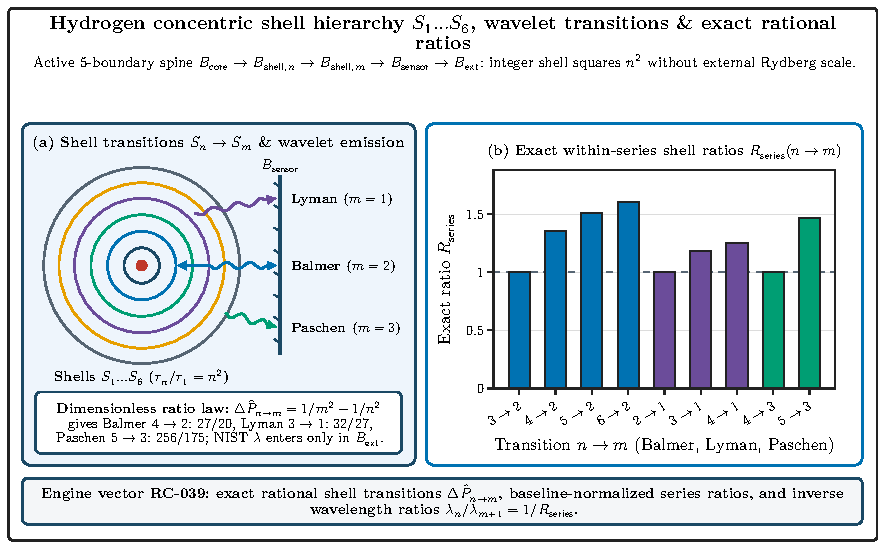
\includegraphics[width=0.92\linewidth,height=0.78\textheight,keepaspectratio]{figures/generated/hydrogen-shell-wavelet-atlas.pdf}
\caption{Concentric hydrogen shell boundaries $S_1\dots S_6$, outgoing Lyman/Balmer/Paschen wavelet packets across $B_{\mathrm{sensor}}$, and exact within-series rational ratios (\texttt{RC-039}, \texttt{hydrogen\_shell\_dec\_transitions.csv}).}
\label{fig:manual-hydrogen-shell-wavelet-atlas}
\end{figure}

\begin{table}[H]
\centering
\caption{Engine-bound exact rational hydrogen shell-transition and wavelet series D.E.C. ledger (\texttt{RC-039}, live from \texttt{hydrogen\_shell\_dec\_transitions.csv}).}
\label{tab:manual-hydrogen-dec-transitions}
{\footnotesize
\begin{tabular}{>{\raggedright\arraybackslash}p{0.112\linewidth}>{\centering\arraybackslash}p{0.092\linewidth}>{\raggedleft\arraybackslash}p{0.116\linewidth}>{\raggedleft\arraybackslash}p{0.116\linewidth}>{\raggedleft\arraybackslash}p{0.116\linewidth}>{\raggedleft\arraybackslash}p{0.124\linewidth}>{\raggedleft\arraybackslash}p{0.124\linewidth}}
\toprule
Series & $n\to m$ & $r_n/r_1=n^2$ & $\Delta\hat{P}_{n\to m}$ & $R_{\mathrm{series}}$ (exact) & $R_{\mathrm{series}}$ (6dp) & $\lambda_n/\lambda_{m+1}$ \\
\midrule
Balmer & 3 $\to$ 2 & 9 & 5/36 & 1 & 1.000000 & 1 \\
Balmer & 4 $\to$ 2 & 16 & 3/16 & 27/20 & 1.350000 & 20/27 \\
Balmer & 5 $\to$ 2 & 25 & 21/100 & 189/125 & 1.512000 & 125/189 \\
Balmer & 6 $\to$ 2 & 36 & 2/9 & 8/5 & 1.600000 & 5/8 \\
Lyman & 2 $\to$ 1 & 4 & 3/4 & 1 & 1.000000 & 1 \\
Lyman & 3 $\to$ 1 & 9 & 8/9 & 32/27 & 1.185185 & 27/32 \\
Lyman & 4 $\to$ 1 & 16 & 15/16 & 5/4 & 1.250000 & 4/5 \\
Paschen & 4 $\to$ 3 & 16 & 7/144 & 1 & 1.000000 & 1 \\
Paschen & 5 $\to$ 3 & 25 & 16/225 & 256/175 & 1.462857 & 175/256 \\
\bottomrule
\end{tabular}
}
\end{table}
